%
% richtungsabl.tex
%
% (c) 2021 Prof Dr Andreas Müller, OST Ostschweizer Fachhochschule
%
\documentclass[tikz]{standalone}
\usepackage{times}
\usepackage{amsmath}
\usepackage{txfonts}
\usepackage[utf8]{inputenc}
\usepackage{graphics}
\usetikzlibrary{arrows,intersections,math}
\usepackage{ifthen}
\begin{document}

\definecolor{darkgreen}{rgb}{0,0.6,0}
\definecolor{rosa}{rgb}{0.8,0.4,0.8}

\newboolean{showgrid}
\setboolean{showgrid}{false}
\def\breite{7}
\def\hoehe{4}

\begin{tikzpicture}[>=latex,thick]
\clip (-6.3,-4.6) rectangle (6.3,4.6);

% Povray Bild
\node at (0,0) {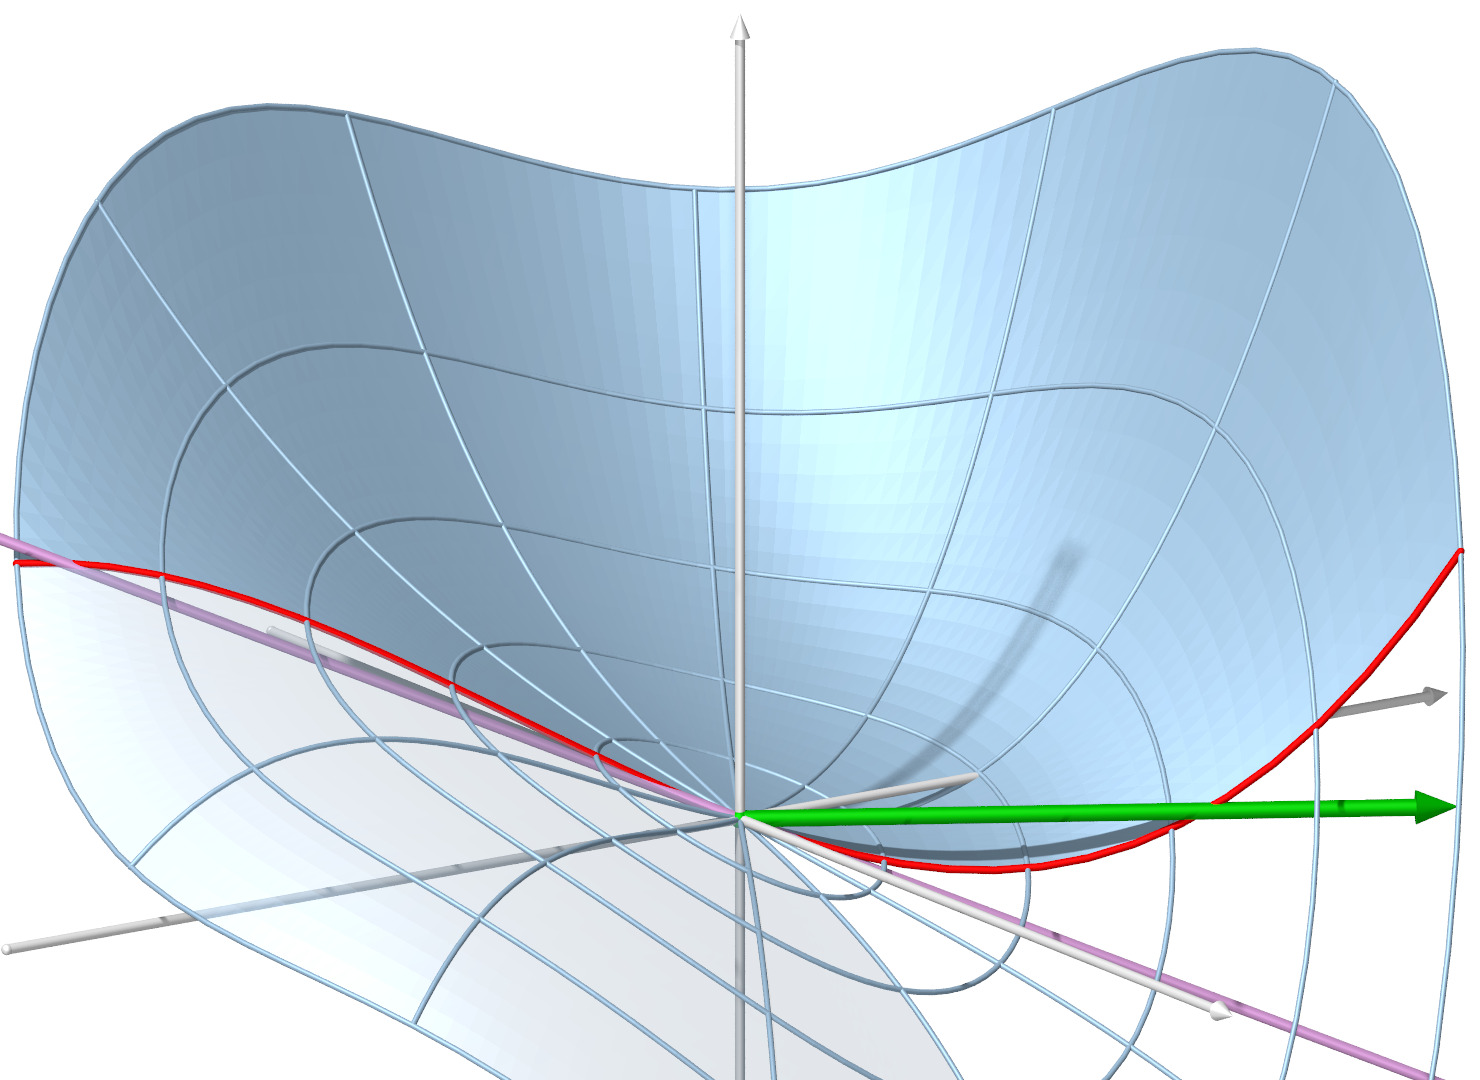
\includegraphics[width=12.6cm]{richtungsabl.jpg}};

% Gitter
\ifthenelse{\boolean{showgrid}}{
\draw[step=0.1,line width=0.1pt] (-\breite,-\hoehe) grid (\breite, \hoehe);
\draw[step=0.5,line width=0.4pt] (-\breite,-\hoehe) grid (\breite, \hoehe);
\draw                            (-\breite,-\hoehe) grid (\breite, \hoehe);
\fill (0,0) circle[radius=0.05];
}{}

\node at (4.0,-4.2) {$x\mathstrut$};
\node at (6.0,-1.0) {$y\mathstrut$};
\node at (-0.2,4.3) {$z\mathstrut$};
\node[color=darkgreen] at (5.9,-2.6) {$\vec{v}$};
\node[color=rosa] at (5.8,-3.8) [below left]
	{$\displaystyle D_{{\color{darkgreen}\vec{v}}} f $};

\node[color=white] at (-4.1,2.7) {$z=f(x,y)$};

\end{tikzpicture}

\end{document}

